%% This is an example first chapter.  You should put chapter/appendix that you
%% write into a separate file, and add a line \include{yourfilename} to
%% main.tex, where `yourfilename.tex' is the name of the chapter/appendix file.
%% You can process specific files by typing their names in at the 
%% \files=
%% prompt when you run the file main.tex through LaTeX.
\chapter{6. Conclusion}

\section{Future Work}
\subsection{a general platform to conduct participatory urban design.}
Current applications like citizens connect is a general purpose app limiting at reporting. 

While it will be useful to have a general app that goes beyond reporting but enables users to propose an intervention, there is a risk that it is hard to maintain the attention for one mobile app. An alternative is to create a framework of the app, which can be customized to specific targets similar to bike lane security and topics discussed in the DISCUSSION section.

Recent web application development have focused on modularising parts to make it easy to reuse and distribute. We can observe this by NPM (Node Package Manager; A software that automates dependency checking and installing parts of software to be used in combination.) Having more than 475,000\footnote{https://www.npmjs.com/} building blocks that one can combine to make web based applications. The elements of one application is modularising as well, were one application are components combined together.

\subsection{safer route navigation}
Utilizing the data collected by the users, we can make a routing system based on safeness within the roads.

Modern map services enables custom path finding, where applications can set different weights for each road segment. Improving the overall bike experience will introduce people to ride their bikes more frequently, causing less cars.
The ring bell Geo location data having weights good and bad, the paths can alter to take a safer route. This will incentives the users for using the app.
In addition, the reported data can be sourced to car navigation systems to let car drivers notice places that are bike heavy.

\subsection{Communal value to Civic value}
Clay Shirkey points out in “Cognitive Surplus.” The internet has lowered the threshold barrier to coordinating with each other, and within this collective action, there are two kinds of value mechanisms; which are Communal and Civic values. Communal value is created by and acknowledged the same group. Although bikebump for urban issues, but is fundamentally for bikers by bikers, which makes bikebump's engine the communal value behavior. Allowing others using different modes of transportation is the next step for inclusion.

\subsection{VR for non bikers}

\begin{marginfigure}[{2cm}]
 	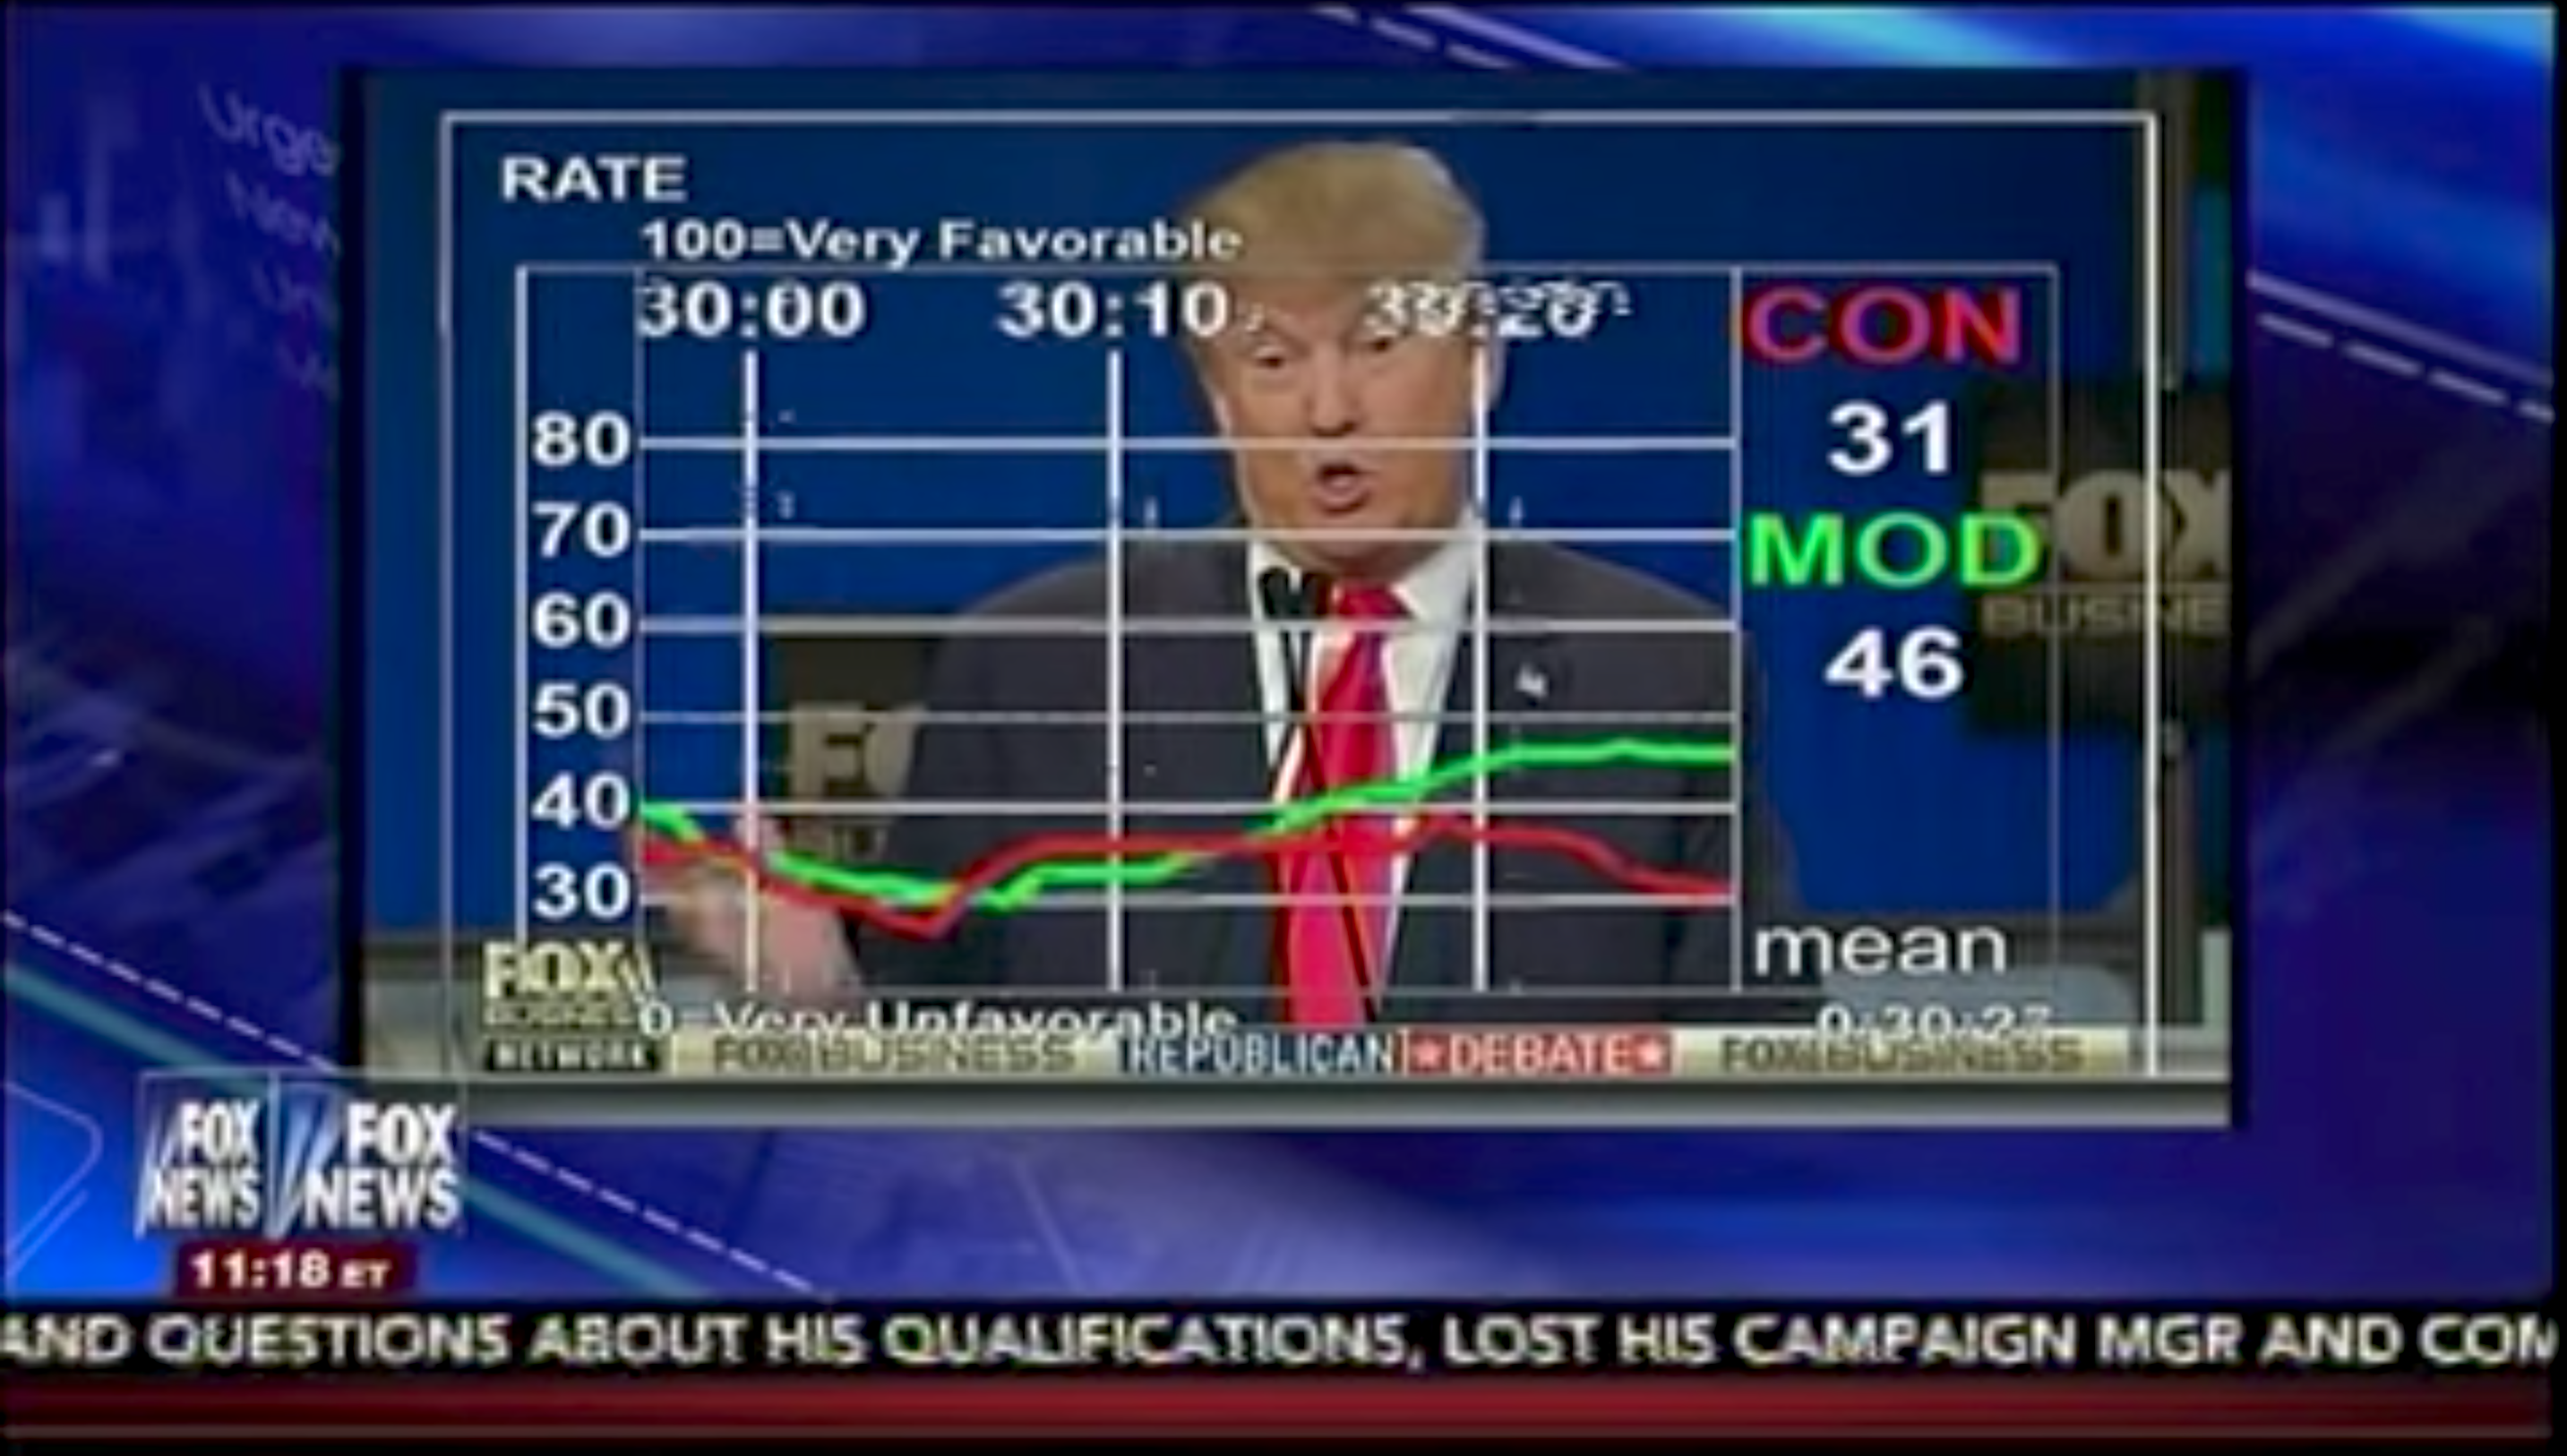
\includegraphics[width=\textwidth]{chapters/6/fig/pollester.png}               
 	 \caption{method for continuous input}
  	\label{fig:poll}
\end{marginfigure}
This app had focused on bikers, and did not take into account people who use other modes of transportation, such as pedestrians or car drivers. It is important to incorporate input from diverse people, and this both applies to the analytical and synthetic phase. It is easy to imagine to discuss the prioritization side, but the data on on-bike reports be should capture in a simulated environment.
Using a VR headset can simulate the bike ride and solicit data from people using a virtual environment projecting recorded material of one commute.




\subsection{How to tackle "relative" valuing}
Multiple people have commented the relativeness of their perception. Data shows that they feel insecure when bike lanes disappear. Using a gradational input like a volume knob will be suitable for getting a continuous input. The users feedback also cast new questions on how to annotate the city. Bikebump used a 15m radius geofence as a method, but users implied that 'good' situations are likely to be a continuous experience rather than a pulsive reaction. Looking at a constant input may also validate this perception.


\subsection{Incentivasation}
Shirkey has mentioned the internet have lowern There are two kinds of value mechanisms in a collective action. \cite{shirky2010cognitive}
distributed donation matching system \\
method for periodic participation - donation matching system \\
% combining for post / pre natural / artificial disasters
\subsection {update infrastructure for autonomous vehicles}
use this renovation opportunity for making cities compatible with autonomous vehicles (PEV)
\subsection{Headphones w/ noise cancellation for collecting sound from both
sides}
% TODO: incomplete
\subsection{Holacracy and liquid democracy}
% TODO: incomplete

\section{Concluding Remarks}
\cite{rudofsky1964architecture}


 